\clearpage
\begin{flushright}
	\textit{Лекция №8}
	\textit{2016.04.11}
\end{flushright}

Cпин блокировки могут использоваться в обработчиках прерывания, а семафоры не могут, так как они переводят поток в состояние ожидания.
Если спин блокировка используется в обработчике прерывания, то перед тем как её захватить где то в другом месте (не в обработчике) необходимо запретить все локальные прерывания, т.е. прерывание на текущем процессоре, иначе может возникнуть следующая ситуация: когда обработчик прерывания прервет выполнение кода ядра, который уже удерживает данную блокировку  и попытается её захватить (при этом блокировка не освобождается, код ядра удерживающий блокировку был вытеснен, но блокировка не освободилась) в это время обработчик прерывания входит в цикл проверки нужной ему блокировки, с другой стороны код ядра, который удерживает блокировку не может возобновить выполнение до тех пор, пока не закончит выполнение обработчик прерывания, естественно он прерывает код ядра, потому что имеет более высокий приоритет. 

Прерывания необходимо запрещать, но только на конкретном процессоре. Если прерывание возникнет на другом процессоре, по отношению к коду ядра, захватившего спин блокировку и обработчик, который выполняется на другом процессоре будет ожидать, то это не приведет к дедлоку, так как процессор, выполняя код ядра сможет освободить спин блокировку. Прерывание должны быть запрещены на локальном процессоре. 

Существует правило блокировки: надо запрещать данные, а не код (т.е. блокировка должна быть связана с данными и защищать их). Ядро предоставляет интерфейс для блокировки и запрета прерываний.

\lstinputlisting[language=c, caption={listing}, label=spinlock_crit_sec]{listing/1.c} 

На однопроцессорной машине код \ref{spinlock_crit_sec} только запретит прерывания.

\paragraph{Отладка спин блокировок}

Для читателей-писателей преимущество отдается писателям. Но если писателей много, то возникнет бесконечное откладывание читателей.
Параметр конфигурации ядра: \verb|CONFIG_DEBUG_SPINLOCK| – подключает несколько отладочных проверок в коде спин блокировок. Например, если указать этот параметр, то в коде будут выполняться проверки на использование неинициализированных спин блокировок, а при освобождении блокировки будет проверяться была ли захвачена блокировка. При тестировании кода всегда следует включать отладку спин блокировок. Чтобы включить дополнительные отладочные средства для спин блокировок можно задать параметр конфигурации ядра \verb|CONFIG_DEBUG_LOCK_ALLOC|.

\section{Семафоры}

Речь идет о семафорах ядра \verb|KERNAL_SEMAPHORES|. В обработчиках прерываний семафоры использовать нельзя. 
В 1 семестре мы изучали семафоры SYSTEM V, там были \verb|get_sem| и \verb|sem_op|, но мы говорим о семафорах ядра. 

Считающий семафор, имеется счетчик заблокированных и очередь потоков, пытающихся захватить данный семафор. На этих семафорах определены 2 операции: down up.

\lstinputlisting[language=c, caption={listing}]{listing/2.c} 

Использование семафоров (по сравнению с спин блокировками)  связано с значительными накладными расходами. 
Если поток ядра заблокирован на семафоре, то ядро может переключиться на выполннеие другой работы, вот и переключение контекста. Когда поток разблокируется, то это связано с переключением контекста.  Получается 2 переключения. Поток владеет аппаратным контекстом.

Из такого поведения семафоров, связанного с переводом процессов в состояние ожидания, можно сделать следующие интересные заключени: \cite{Lav_Linux_kernel}
\begin{enumerate}
	\item Так как задания, которые конфликтуют при захвате блокировки, переводятся в состояние ожидания и в этом состоянии ждут, пока блокировка не будет освобождена, семафоры хорошо подходят для блокировок, которые могут удерживаться в течение длительного времени.
	\item Так как поток выполнения во время конфликта при захвате блокировки находится в состоянии ожидания, то семафоры можно захватывать только в контексте процесса. Контекст прерывания планировщиком не управляется.
	\item  При захвате семафора нельзя удерживать спин-блокировку, поскольку процесс может переходить в состояние ожидания, ожидая на освобождение семафора, а при удержании спин-блокировки в состояние ожидания переходить нельзя.
	\item Семафоры не запрещают приемтивность ядра. Код который удерживает семафор может быть вытеснен.  Следствием этого является то, что семафоры не влияют на латентность планировщика. (При удержании семафора (хотя разработчик может и не очень хотеть этого) процесс может переходить в состояние ожидания. Это не может привести к тупиковой ситуации, когда другой процесс попытается захватить блокировку (он просто переходит в состояние ожидания, что в конце концов дает возможность выполняться первому процессу).)
	\item Cемафоры позволяют удерживать их любому кол-ву потоков.  Кол-во потоков, которые одновременно могут удерживать семафор определяются счетчиком использования при создании семафора.
	\item Спин блокировку может удерживать только один процесс/поток. Семафоры в ядре используются мало.
\end{enumerate}

\section{Условные переменные}

Completion variable – средство синхронизации двух задач, когда одна задача сообщает другой задаче что переходит в состояние ожидания, пока другая задача не выполнит какую-нибудь работу. Условные переменные описываются структурой, которая определена в файле $linux/completion.h$.
Статическая условная переменная создается с помощью макроса \verb|DECLARE_COMPLETION(mr_com);|.
Для динамического создания используется функция \verb|init_completion();| 

\begin{lstlisting}[language=c, caption=Функции для работы с условными переменными]
init_completion(struct completion *); 

//ждет сигнала
wait_for_completion(struct completion *);

//отправляет сигнал всем ожидающим сигналам, тем самым активируя их к выполненияю
complete(struct completion *);
\end{lstlisting}

\paragraph{Задачу производство потребление (задача ограниченного буфера)}

потребитель запускается после всех ???. 

\begin{figure}[H]
  \centering
  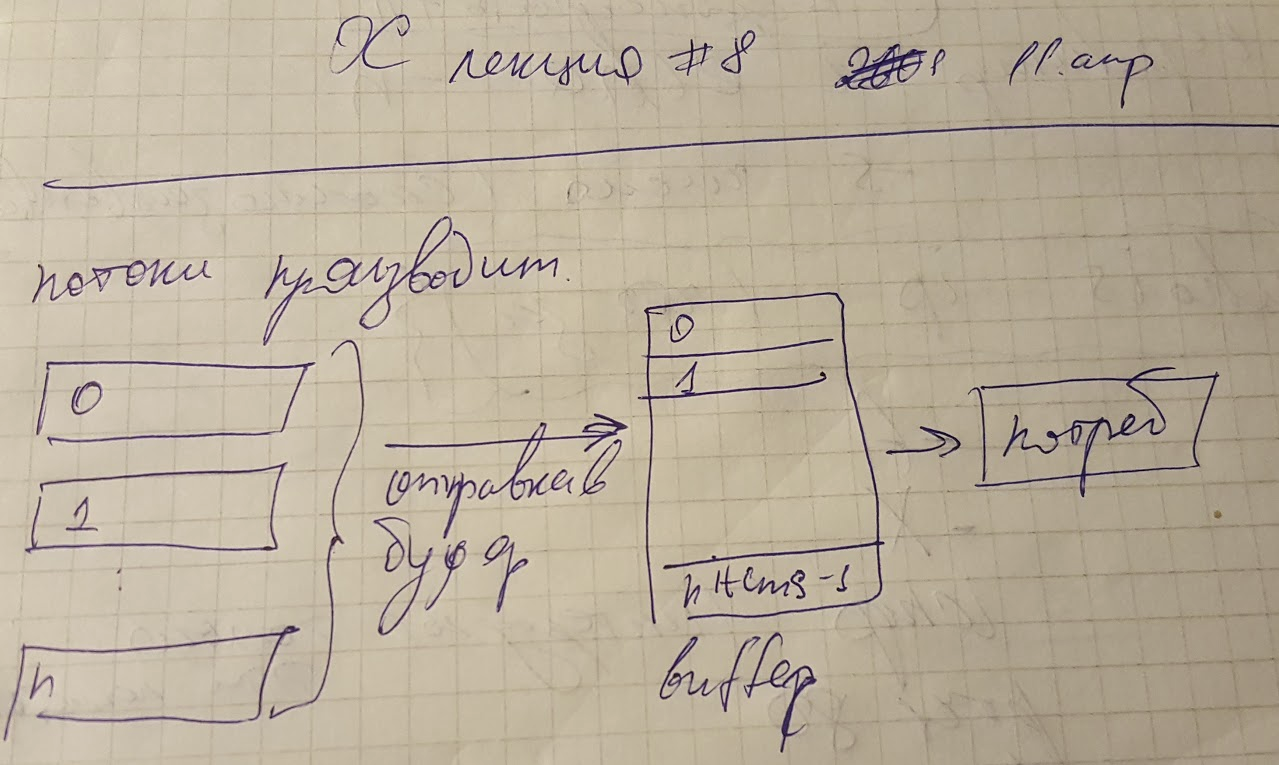
\includegraphics[width=\textwidth]{pic/1.png}
  \caption{pic}
\end{figure}

\lstinputlisting[language=c, caption={listing}, label=code_prod_cons]{listing/3.c} 

В \ref{code_prod_cons} есть мьютексы, они также используются наряду с семафорами, и в \verb|pthread_cond_signal| использующую условную переменную. Если буфер был пуст, то естественно потребителю взять нечего, соответственно в момент помещения в него значения вызывается функция сигнал \verb|pthread_cond_signal|. Этот сигнал разблокирует любой процесс, который ожидает.
